%===============================================================
% Utilize este template para construir apresentações da Especialização em Eng. Ferroviária na Faeng-UFMT.
% Atente-se para a estrutura deste arquivo:
%   Linhas 1-281: Configurações do template. Não altere!
%   Linhas 282-299: Definições do autor. Altere apenas seu nome,  
%                   seu curso, nome do orientador, data de
%                   apresentação e título.
%  A partir da linha 300: Corpo da apresentação.
%===============================================================

\documentclass{beamer}
\usepackage[utf8]{inputenc}
%\usepackage{lmodern}
\usepackage{comment}
\usetheme{Madrid}
  \usepackage[maxbibnames=99]{biblatex}
\definecolor{cvut_navy}{HTML}{0065BD}
\definecolor{cvut_blue}{HTML}{6AADE4}
\definecolor{cvut_gray}{HTML}{156570}
\definecolor{faeng_blue}{HTML}{09246F}
\usepackage{biblatex}
%\usepackage{tikz}
%\usepackage{pgfplots}
\usepackage[makeroom]{cancel}
\usepackage{threeparttable}
\usepackage[utf8]{inputenc}
%\usepackage[usenames,dvipsnames]{xcolor}
%\addbibresource{biblatex-examples.bib}
%\setbeamercolor{section in toc}{}
\setbeamercolor{section in toc}{fg=black,bg=yellow} 
\setbeamercolor{alerted text}{fg=cvut_blue}
\usepackage{tikzsymbols}
\usepackage{textcomp}
\usepackage{parskip}
\definecolor{darkblue}{rgb}{0, 0, 0.5} 
\definecolor{babyblue}{rgb}{0.54, 0.81, 0.94}
\usepackage{pgf}
\usepackage[backend=biber]{biblatex}
\addbibresource{ref.bib}

%\usepackage{pythontex} 
\usepackage{tcolorbox}
\tcbuselibrary{skins}
\usepackage{minted}
\usepackage{hyperref}
\usepackage{xcolor,soul}
\definecolor{lightblue}{rgb}{.90,.95,1}
\sethlcolor{lightblue}
\renewcommand<>{\hl}[1]{\only#2{\beameroriginal{\hl}}{#1}}
\setbeamertemplate{page number in head/foot}[totalframenumber]
%%% attravive box over equestion
\usepackage{empheq}
\usepackage{xcolor}
\definecolor{lightgreen}{HTML}{90EE90}
\newcommand{\boxedeq}[2]{\begin{empheq}[box={\fboxsep=6pt\fbox}]{align}\label{#1}#2\end{empheq}}
\newcommand{\coloredeq}[2]{\begin{empheq}[box=\colorbox{lightgreen}]{align}\label{#1}#2\end{empheq}}
\newcommand{\highlight}[1]{%
  \colorbox{red!40}{$\displaystyle#1$}}

  \definecolor{babyblue}{rgb}{0.54, 0.81, 0.94}
\definecolor{babypink}{rgb}{0.96, 0.76, 0.76}
\definecolor{blue(ncs)}{rgb}{0.0, 0.53, 0.74}
\definecolor{pistachio}{rgb}{0.58, 0.77, 0.45}
\definecolor{darksalmon}{rgb}{0.91, 0.59, 0.48}
\definecolor{lightsalmonpink}{rgb}{1.0, 0.6, 0.6}
\definecolor{columbiablue}{rgb}{0.61, 0.87, 1.0}
\definecolor{corn}{rgb}{0.98, 0.93, 0.36}
\definecolor{jonquil}{rgb}{0.98, 0.85, 0.37}
\definecolor{bananayellow}{rgb}{1.0, 0.88, 0.21}
\newcommand{\bert}{\ensuremath{%
  \mathchoice{\includegraphics[height=2ex]{Bert-pic-removebg-preview.png}} 
    {\includegraphics[height=2ex]{Bert-pic-removebg-preview.png}}
    {\includegraphics[height=1.5ex]{Bert-pic-removebg-preview.png}}
    {\includegraphics[height=1ex]{Bert-pic-removebg-preview.png}}
}}
\newcommand{\Tr}{\operatorname{Tr}}
\newcommand{\Arg}{\operatorname{Arg}}
\useoutertheme{infolines}
\newtcbox{\boxedeqn}{
  nobeforeafter,
  colframe=red!70!black,
  colback=red!5,
  boxrule=0.5pt,
  arc=4pt,
  boxsep=5pt,
  left=5pt,
  right=5pt,
  top=5pt,
  bottom=5pt,
}
\usepackage{courier}
%\usepackage{animate}  
\usepackage{expl3}
%\usepackage[listings,theorems]{tcolorbox}

%%%%%%%%%%%%%%%%%%%%%%%%%%%%%%%%%%%%%%%%%%%%%%%%%%%%%%%%%%%%%%%%%%%%%  
%commands for simulating terminal in/output  
%\scroll[<line separator string>]{<width as TeX dim>} 
%                             {<number of lines>}{terminal text line}  
%\clearbuf  %clears line buffer  
%%%%%%%%%%%%%%%%%%%%%%%%%%%%%%%%%%%%%%%%%%%%%%%%%%%%%%%%%%%%%%%%%%%%%  

\newcommand\scroll[4][§§]{
  \seq_set_split:Nnn\g_inputline_seq{#1}{#4}
  \seq_map_inline:Nn\g_inputline_seq{
    \seq_gput_right:Nx\g_linebuffer_seq{##1}
    \int_compare:nT{\seq_count:N\g_linebuffer_seq>#3}{
      \seq_gpop_left:NN\g_linebuffer_seq\dummy
    }
  }
  \fbox{\begin{minipage}[t][#3\baselineskip]{#2}
    \ttfamily
    \seq_map_inline:Nn\g_linebuffer_seq{\mbox{##1}\\}
  \end{minipage}}
}
\newcommand\clearbuf{\seq_gclear:N\g_linebuffer_seq}
\ExplSyntaxOff

\setbeamertemplate{headline}{%
\begin{beamercolorbox}[colsep=1.5pt]{upper separation line head}
\end{beamercolorbox}
\begin{beamercolorbox}{section in head/foot}
    \vskip2pt\insertsectionnavigationhorizontal{\paperwidth}{}{\hskip0pt plus1filll}\vskip2pt
\end{beamercolorbox}%

\begin{beamercolorbox}[colsep=1.5pt]{lower separation line head}
\end{beamercolorbox}
}
\makeatletter
\newcommand\SoulColor{%
  \let\set@color\beamerorig@set@color
  \let\reset@color\beamerorig@reset@color}
\makeatother
\SoulColor
\usepackage{amsmath, bm}
\usepackage{tikz}
\setbeamercovered{dynamic}

\newcommand{\highlightt}[1]{%
  \colorbox{blue!40}{$\displaystyle#1$}}

\newenvironment<>{problock}[1]{%
  \begin{actionenv}#2%
      \def\insertblocktitle{#1}%
      \par%
      \mode<presentation>{%
       % \setbeamercolor{block title}{fg=white,bg=orange!20!black}
        %\setbeamercolor{block title}{fg=white,bg=red!10!black}
        \setbeamercolor{block title}{fg=white,bg=babyblue}
       \setbeamercolor{block body}{fg=black,bg=white!50}
       \setbeamercolor{itemize item}{fg=orange!20!black}
       \setbeamertemplate{itemize item}[triangle]
     }%
      \usebeamertemplate{block begin}
    \par\usebeamertemplate{block end}
    \end{actionenv}
    }
    
    \newcommand<>{\uncovergraphics}[2][{}]{
    % Taken from: <https://tex.stackexchange.com/a/354033/95423>
    \begin{tikzpicture}
    \node[anchor=south west,inner sep=0] (B) at (4,0)
        {\includegraphics[#1]{#2}};
    \alt#3{}{%
        \fill [draw=none, fill=background, fill opacity=0.9] (B.north west) -- (B.north east) -- (B.south east) -- (B.south west) -- (B.north west) -- cycle;
    }
    \end{tikzpicture}
}

\newlength\dlf
\newcommand\alignedbox[3][yellow]{
  % #1 = color (optional, defaults to yellow)
  % #2 = before alignment
  % #3 = after alignment
  &
  \begingroup
  \settowidth\dlf{$\displaystyle #2$}
  \addtolength\dlf{\fboxsep+\fboxrule}
  \hspace{-\dlf}
  \fcolorbox{red}{#1}{$\displaystyle #2 #3$}
  \endgroup
}

\usepackage{collcell}
\usepackage{booktabs}
\usepackage{etoolbox}
%\usepackage{remreset}% tiny package containing just the \@removefromreset command
\makeatletter

\usepackage{xcoffins}
\NewCoffin\tablecoffin
\NewDocumentCommand\Vcentre{m}
  {%
    \SetHorizontalCoffin\tablecoffin{#1}%
    \TypesetCoffin\tablecoffin[l,vc]%
  }
  
\usepackage{pgfpages}

%% Important 
%%% show note or disable note. 
%\setbeameroption{show notes on second screen=right} % Both

\setbeamertemplate{note page}{\pagecolor{gray!5}\insertnote}\usepackage{palatino}
\usepackage{xcolor}
\usepackage{soul}
\usepackage{etoolbox}
\makeatletter
%\patchcmd{\slideentry}{\ifnum#2>0}{\ifnum2>0}{}{\@error{unable to patch}}% replace the subsection number test with a test that always returns true
\makeatother

%\setbeamercolor*{palette primary}{bg=cvut_navy,fg=gray!20!white}
\setbeamercolor*{palette primary}{bg=faeng_blue,fg=gray!20!white}
\setbeamercolor*{palette secondary}{bg=faeng_blue,fg=gray!20!white} % no color
%\setbeamercolor*{palette secondary}{bg=cvut_navy,fg=cvut_navy}
%\setbeamercolor*{palette secondary}{bg=cvut_blue,fg=white}
\setbeamercolor*{palette tertiary}{parent=palette primary} % color of the top and date
\setbeamercolor*{palette quaternary}{fg=faeng_blue,bg=gray!5!white}
\setbeamercolor*{sidebar}{fg=faeng_blue,bg=gray!15!white}
\usepackage[first=0,last=9]{lcg}
\newcommand{\ra}{\rand0.\arabic{rand}}
\usepackage{color, colortbl}
\usepackage{stackengine,tikz}
\usepackage{transparent}
\usepackage{pgfpages}
\usepackage{graphicx}% http://ctan.org/pkg/graphicx
\usepackage{booktabs}% http://ctan.org/pkg/booktabs
\colorlet{Gray}{gray!30}    
\newcommand*{\MinNumber}{0}%
\newcommand*{\MaxNumber}{0.4}%
\definecolor{bubblegum}{rgb}{0.99, 0.76, 0.8}
\newcommand{\ApplyGradient}[1]{%
  \pgfmathsetmacro{\PercentColor}{100.0*(#1-\MinNumber)/(\MaxNumber-\MinNumber)}%
  \edef\x{\noexpand\cellcolor{babyblue!\PercentColor}}\x\textcolor{black}{#1}%
}
\newcolumntype{R}{>{\collectcell\ApplyGradient}{c}<{\endcollectcell}}

\setbeamercolor{titlelike}{parent=palette primary}
\setbeamercolor{frametitle}{parent=palette primary}

\setbeamercolor{B}{bg=red!30,fg=black}

\setbeamertemplate{section in toc}[default]
\setbeamercolor{itemize item }{fg=blue}
\setbeamertemplate{itemize item}[circle]

\setbeamercolor*{separation line}{}
\setbeamercolor*{fine separation line}{}

\setbeamertemplate{navigation symbols}{} 
\setbeamertemplate{caption}{\raggedright\insertcaption\par}

\setbeamercolor*{block title example}{fg=white,bg=purple!75!black}
\setbeamercolor*{block body example}{fg= black, bg= white}

\setbeamercolor{itemize item}{fg=cvut_navy} % all frames will have red bullets
\setbeamercolor{block title}{bg=red!30,fg=black}
\setbeamertemplate{subsection in toc}[subsections numbered]

\usepackage{eqnarray,amsmath}
\usepackage{amsfonts}
\usepackage{amssymb}
\usefonttheme{professionalfonts}
\usepackage{graphicx}
\usepackage{booktabs} 
\usepackage{bm}
\usepackage{mathtools}
\usepackage[utf8]{inputenc}
\usepackage[T1]{fontenc}
\usepackage[french]{babel}
\usepackage{lmodern} 
\usepackage{booktabs}

\setbeamercolor{block title}{fg=black, bg=yellow}
\setbeamercolor{block2}{use=structure,fg=white,bg=purple!75!black}
% definice makra
\def\bq{\mbox{\kern.1ex\protect\raisebox{-1.3ex}[0pt][0pt]{''}\kern-.1ex}}
\def\eq{\mbox{\kern-.1ex``\kern.1ex}}
\def\ifundefined#1{\expandafter\ifx\csname#1\endcsname\relax }%
\ifundefined{uv}%
        \gdef\uv#1{\bq #1\eq}
\fi

\usepackage{algpseudocode}
\usepackage{ragged2e}
\usepackage{csquotes}

\usepackage{memhfixc}

%====================================================
%========== DEFINITION OF AUTHORS ETC...=============
%====================================================

\author[CentraleSupélec - 2A]{EI - Contrôle de la pollution acoustique}
\institute[]{
    CentraleSupélec - 2A \\  
    Université Paris-Saclay \\ 
    \vspace{1mm} \\ 
    \textbf{Auteurs:}  \\ 
	Moghit Yebari \\
    Yi Zhong \\
	Farouk Yartaoui \\
    Nabil Alami \\
    Raphaël Pain Dit Hermier \\
    Edward Lucyszyn
}

\title[Soutenance d'EI]{Optimisation de la répartition d'un matériau absorbant}

\date[\today]{\small{\today}}

%====================================================
%========== BEGINNING OF DOCUMENT ===================
%====================================================

\begin{document}

\begin{frame}[plain]
	\titlepage
	\begin{center}%
  		
\includegraphics[height=1.5cm]{Beamer/logo.png}
	\end{center}
\end{frame}

\begin{frame}[plan]{Sommaire}
\tableofcontents[]
%\note[item]{note here }
\end{frame}

% =========================================

\section{Introduction}

\begin{frame}{}
    \begin{center}
        \Huge \textcolor{faeng_blue}{Introduction} 
    \end{center}
\end{frame}
\begin{frame}{Introduction}

\begin{figure}
        \centering
        
\includegraphics[width=0.5\linewidth]{Beamer/Onera-bloc-marque.png}
    
    \end{figure}
• Projet d'EI en collaboration avec l’ONERA.\\


• Le but : étudier la pollution acoustique générée dans un réacteur d’avion \\

• Deux parties : Théorique \& Numérique
\end{frame}


\section{Partie théorique}

\begin{frame}{}
    \begin{center}
        \Huge \textcolor{faeng_blue}{Partie théorique} 
    \end{center}
\end{frame}

\begin{frame}{Problème initial}
    Le problème initial  :
    \[
    (P) \hspace{2pt} : \hspace{2pt}
    \begin{cases}
    \displaystyle \Delta p + k_0^2\Big(1 - \frac{iM_0}{k_0}\frac{\partial}{\partial x}\Big)^2p = f \in L^2(\Omega) \hfill \\
    \displaystyle Z\frac{\partial p}{\partial n} + ik_0Z_0\chi \Tr \Bigl[ \Bigl(1-i \frac{M_0}{k_0} \Big(\frac{\partial}{\partial x} + \textcolor{blue}{\frac{\partial}{\partial y}}\Big) \Bigr)^2p \Bigr] = 0$ sur \Gamma = \Gamma_1 \sqcup \Gamma_2 \hspace*{2cm} \hfill
    \\
    \displaystyle \Tr(p) = g $ sur $ \Gamma_{in} \hfill \\
     \displaystyle \frac{\partial p}{\partial n} + ik \Tr(p) = 0 $ sur $\Gamma_{out} \hfill    
    \end{cases}
\]

avec $\displaystyle Z_0 \in \mathbb{R}$,  $Z \in \{z \in \mathbb{C} \hspace{2pt} | \hspace{2pt} Re(z) > 0\}$, $\chi : \Gamma \to \{0,1\} $, $\displaystyle M_0 = \frac{u_0}{c_0}$, $\displaystyle k_0 = \frac{\omega}{c_0}$, $\displaystyle k = \frac{\omega}{u_0}$.

\end{frame}
\begin{frame}{Formulation variationnelle}
    Une "double" intégration par partie
    
    \begin{equation} \displaystyle
    \begin{cases}
    \displaystyle \int_{\Gamma} \Tr \Bigr(\frac{\partial^2 p}{\partial x^2}\Bigl) \Tr(\overline{q}) \chi \hspace{2pt} d\mu = - \int_{\Gamma} \Tr \Bigl( \frac{\partial p}{\partial x} \Bigr) \Tr \Bigl( \frac{\partial \overline{q}}{\partial x}\Bigr)\chi d\mu \nonumber \\

    \displaystyle \int_{\Gamma} \Tr \Bigr(\frac{\partial^2 p}{\partial y^2}\Bigl) \Tr(\overline{q})\chi \hspace{2pt} d\mu = - \int_{\Gamma} \Tr \Bigl( \frac{\partial p}{\partial y} \Bigr) \Tr \Bigl( \frac{\partial \overline{q}}{\partial y}\Bigr)\chi d\mu \\

    \displaystyle \int_{\Gamma} \Tr \Bigr(\frac{\partial^2 p}{\partial x \partial y}\Bigl) \Tr(\overline{q}) \chi \hspace{2pt} d\mu = - \int_{\Gamma} \Tr \Bigl( \frac{\partial p}{\partial x} \Bigr) \Tr \Bigl( \frac{\partial \overline{q}}{\partial y}\Bigr) \chi d\mu\\

    \displaystyle \int_{\Gamma} \Tr \Bigr(\frac{\partial^2 p}{\partial x \partial y}\Bigl) \Tr(\overline{q}) \chi \hspace{2pt} d\mu = - \int_{\Gamma} \Tr \Bigl( \frac{\partial p}{\partial y} \Bigr) \Tr \Bigl( \frac{\partial \overline{q}}{\partial x}\Bigr) \chi d\mu
    \end{cases}
\end{equation}

\end{frame}
\begin{frame}{Formulation variationnelle}
\small
    \begin{equation}
\label{eq:FV}
A(p,q) = l(q) \nonumber
\end{equation}
où
\scriptsize \[A(p,q) = (\nabla p, \nabla q)_{(L^2(\Omega))^2} + ik(\Tr(p),\Tr(q))_{L^2(\Gamma_{out})} + C(p,q) -k_0^2(p,q)_{L^2(\Omega)}\]
\[+ 2iM_0k_0\Big(\frac{\partial p}{\partial x}, q\Big)_{L^2(\Omega)} -M_0^2\Big(\frac{\partial p}{\partial x},\frac{\partial q}{\partial y}\Big)_{L^2(\Omega)}+ M_0^2\Big(\frac{\partial p}{\partial x}\cdot n_x,\Tr(q)\Big)_{B'(\partial \Omega),B(\partial \Omega)}\]
puis
\[l(q) = -(\Tilde{f},q)_{L^2(\Omega)}\]
avec
\[C(p,q) = -ik_0\frac{Z_0}{Z} \biggl[ \int_{\Gamma} \Tr(p) \Tr(\overline{q}) \hspace{2pt} \chi \hspace{2pt} d\mu - 2i\frac{M_0}{k_0} \int_{\Gamma} \Tr \Bigl( \frac{\partial p}{\partial x}+\frac{\partial p}{\partial y} \Bigr) \Tr(\overline{q}) \hspace{2pt} \chi \hspace{2pt} d\mu +\]
\[\frac{M_0^2}{k_0^2}\int_{\Gamma} \Tr \Bigl( \frac{\partial p}{\partial x}+\frac{\partial p}{\partial y}\Bigr)\Tr\Bigl( \frac{\partial \overline{q}}{\partial x}+\frac{\partial \overline{q}}{\partial y}\Bigr) \hspace{2pt} \chi  \hspace{2pt} d\mu \biggl].\]
\end{frame}


\begin{frame}{Première approche de l'espace des solutions}
    • \small On veut imposer sur $V(\Omega)$ que $\displaystyle \Tr(q)_{|\Gamma_{in}} = 0$ pour bénéficier de l'inégalité de Poincaré.
    
    • Il faut de plus $\displaystyle \frac{\partial q}{\partial x},\frac{\partial q}{\partial y}\in H^1(\Omega)$. On pose alors :
    \footnotesize \[V(\Omega)=\{q \in H^1(\Omega), \Tr(q)=0 \text{ sur } \Gamma_{in}, \frac{\partial q}{\partial x}, \frac{\partial q}{\partial y} \in H^1(\Omega) \} = H^2(\Omega) \cap (\Tr^{|\Gamma_{in}})^{-1}(\{0\}).\]
    \[\|q\|_{V(\Omega)}^2:= \|q\|_{H^2(\Omega)}^2 - \|q\|_{L^2(\Omega)}^2.\]

    • \small  $V(\Omega) = Ker(\Tr^{|\Gamma_{in}}\circ \iota)$\\ 


    $\to$ $(V(\Omega), \|\cdot\|_{V(\Omega)})$ est un espace de Hilbert.
\end{frame}
\begin{frame}{Deuxième approche de l'espace des solutions}
    Approche précédente : insuffisante pour résoudre le caractère bien posé
    
    $\to$ " Agrandir notre espace de solutions "

On dit alors qu'une fonction $v\in H^1(\Omega)$ est dans l'espace des solutions $V(\Omega)$ si elle vérifie:

\begin{equation}
\label{eq:soleq}
    \begin{cases}
    \displaystyle \Delta q = \varphi \in L^2(\Omega) \hfill 
    \\
    \displaystyle Z\frac{\partial q}{\partial n} + ik_0Z_0\chi \Tr(q) = \psi \in L^2(\Gamma) \hfill \hspace{45pt} 
    \\
    \displaystyle \Tr(q) = 0 \text{ sur } \Gamma_{in} \hfill 
    \\
    \displaystyle \frac{\partial q}{\partial n} + ik \Tr(q) = 0 \text{ sur } L^2(\Gamma_{out}) \hfill 
    \end{cases} 
\end{equation}




\end{frame}

\begin{frame}{Deuxième approche de l'espace des solutions}
    On peut alors réexprimer les solutions de (\ref{eq:soleq}) par la formulation variationnelle :
    \[\forall h\in V(\Omega), A^*(q,h) = l^*(\varphi,\psi,h)\]

    On pose alors \small$\displaystyle V(\Omega) = \{q\in H^1(\Omega), \exists (\varphi,\psi)\in L^2(\Omega)\times L^2(\Gamma), \forall h\in V(\Omega), A^*(q,h) = l^*(\varphi,\psi,h)\}$, muni de la norme $\displaystyle \|\cdot\|_{V(\Omega)}:= \|\nabla \cdot\|_{(L^2(\Omega))^2}$. \\

• Le problème variationnel devient :
\[\forall h\in V(\Omega), ((Id-K)q,h)_{V(\Omega)} = (A_{\psi}\psi+A_{\varphi}\varphi, h)_{V(\Omega)}\]
Ce qui revient donc à résoudre $(Id-K)q = A_{\psi}\psi+A_{\varphi}\varphi$ sur $V(\Omega)$\\

$\to$ \textcolor{blue}{\textbf{Théorème Fredholm}} : $(V(\Omega), \|\cdot\|_{V(\Omega)})$ est un espace de Hilbert.
\end{frame}
\begin{frame}{Caractère bien posé}
     • Norme équivalente sur $V(\Omega)$ ($M_0 < 1$): 
        \[(\|q\|'_{V(\Omega)})^2:= \|\nabla q\|_{(L^2(\Omega))^2}^2 - M_0^2\Big\|\frac{\partial q}{\partial x}\Big\|_{L^2(\Omega)}^2+\Big\|\Tr\Big(\frac{\partial q}{\partial x}+\frac{\partial q}{\partial y}\Big)\Big\|_{L^2(\Gamma)}^2.\]
    • Décomposition de type Fredholm de $A(p,q)$:
    \[A(p,q) = \Theta(p,q) + \xi(p,q)\]

    • On montre $\Theta$ coercive \cite{2} et $\xi(p,q)= (\Xi p,q)_{V(\Omega)}$ avec $\Xi$ compact 
    
\end{frame}

\begin{frame}{Énergie}
    • Énergie : \begin{center}
        $J= \int_{\Omega} |p(\chi)|^2 dx \hspace{2pt}$
    \end{center}

    \[ U_{\text{ad}}(\beta) = \left\{\chi \in L^{\infty}(\Gamma) \, \middle| \, \forall x \in \Gamma, \chi(x) \in \{0,1\}, 0 < \beta = \int_{\Gamma} \chi \, d\mu < \mu(\Gamma)\right\} \]

    \[ U_{\text{ad}}^*(\beta) = \left\{\chi \in L^{\infty}(\Gamma) \, \middle| \, \forall x \in \Gamma, \chi(x) \in [0,1], 0 < \beta = \int_{\Gamma} \chi \, d\mu < \mu(\Gamma)\right\} \]

    L'ensemble \(U_{ad}^*(\beta)\) est compact dans \(L^\infty(\Gamma)\) pour la convergence faible*.

    $\to$ On souhaite montrer la continuité de l'énergie par rapport à $\chi$

\end{frame}

\begin{frame}{Étude de l'énergie}
• Soit $\chi_m \stackrel{\ast}{\rightharpoonup} \chi$ dans $L^\infty(\Gamma)$ .

• $p_m$ correspond à la solution de $(P_H)$ pour $\chi_m$ et $p$ celle pour  $\chi$.
Alors \textcolor{blue}{$v_m = p_m - p $} est solution de :\\
\small\[
    (P_{H,m}) \hspace{2pt} : \hspace{2pt}
    \begin{cases}
    \displaystyle \Delta v_m + k_0^2\Big(1 - \frac{iM_0}{k_0}\frac{\partial}{\partial x}\Big)^2v_m = 0 \\
    \displaystyle Z\frac{\partial v_k}{\partial n} + ik_0Z_0\chi_k \Tr \Bigl[ \Bigl(1-i \frac{M_0}{k_0} \Big(\frac{\partial}{\partial x} + \frac{\partial}{\partial y}\Big) \Bigr)^2v_m \Bigr] = h_m \text{ sur } \Gamma 
    \\
    \displaystyle \Tr(v_m) = 0 \text{ sur }\Gamma_{in} \hfill \\
    \displaystyle \frac{\partial v_m}{\partial n} + ik \Tr(v_m) = 0 \text{ sur } \Gamma_{out} \hfill
    \end{cases} 
\]\\

où $h_k = \displaystyle - ik_0Z_0(\chi_m - \chi)\Tr \Bigl[ \Bigl(1-i \frac{M_0}{k_0} \Big(\frac{\partial}{\partial x} + \frac{\partial}{\partial y}\Big) \Bigr)^2p \Bigr]$
    
\end{frame}

\begin{frame}{Étude de l'énergie}
    • $v_m$ est borné dans $V(\Omega)$ qui est de Hilbert\\
    
    • $\exists (v_{m_j})_{j \in \mathbb{N}} \subset (v_m)_{m \in \mathbb{N}}$ et $v \in V(\Omega) : v_{m_j} \rightharpoonup v$ dans $V(\Omega)$.\\

    • \small $\lVert v_{m_j} \rVert^2_{V(\Omega)}\leq C_1 \Big|\int_{\Gamma} k_0Z_0(\chi_{m_j} - \chi)\Tr \Bigl[ \Bigl(1-i \frac{M_0}{k_0} \Big(\frac{\partial}{\partial x} + \frac{\partial}{\partial y}\Big) \Bigr)^2p \Bigr] \overline{\Tr(v_{m_j})}d\mu\Big|$\\

    • On montre ainsi que $0$ est l'unique valeur d'adhérence faible de la suite $(v_m)$, puis que $v = 0$\\

    • On montre que la convergence est même forte\\
    
\begin{center}
    \large $\to$ \textcolor{red!80!black}{continuité de $J^*$ sur $U_{ad}^*(\beta)$.}
\end{center}
    
\end{frame}

\begin{frame}{Énergie et Lagrangien}
    \[
L(\chi, w, q) = F_V(\chi, w, q) + J(w), \quad \forall w, q \in H
\]

\[
\langle J'(\chi), \chi_0 \rangle = \langle \frac{\partial L (\chi, u(\chi), p(\chi))}{\partial \chi}, \chi_0 \rangle
\]
• Problème adjoint :
\small \[
\langle \frac{\partial L}{\partial u_R}, \phi_R \rangle &= 0 \quad \forall \phi_R \in V(\Omega) \]\\
\[
\langle \frac{\partial L}{\partial u_I}, \phi_I \rangle &= 0 \quad \forall \phi_I \in V(\Omega)\]

\end{frame}

\begin{frame}{Énergie et Lagrangien}
    \small
    \[\langle J'(\chi), \chi_0\rangle = \]
    \[k_0\frac{Z_0}{|Z|^2}\Re e\Big( \Bar{Z}\biggl[ \int_{\Gamma} \Tr(p(\chi_0)) \Tr(\Bar{q}(\chi_0))\chi_0 d\mu \]
    \[-2i\frac{M_0}{k_0} \int_{\Gamma} \Tr \Bigl( \frac{\partial p(\chi_0)}{\partial x}+\frac{\partial p(\chi_0)}{\partial y} \Bigr)\Tr(\Bar{q}(\chi_0))\chi_0 \hspace{2pt} d\mu\]
    \[ -\frac{M_0^2}{k_0^2}\int_{\Gamma} \Tr \Bigl( \frac{\partial p(\chi_0)}{\partial x}+\frac{\partial p(\chi_0)}{\partial y}\Bigr)\Tr\Bigl( \frac{\partial \overline{q}(\chi_0)}{\partial x}+\frac{\partial \overline{q}(\chi_0)}{\partial y}\Bigr) \hspace{2pt} \chi_0  \hspace{2pt} d\mu\biggr ]\Big) \]\\ \normalsize

    \[
    \boxedeqn{\langle J'(\chi), \chi_0\rangle = \Re e(iC(p(\chi_0),q(\chi_0),\chi_0))}
    \]
    
\end{frame}

\begin{frame}{Conclusion théorique}
    • Objectif principal : existence d'une distribution optimale 
    $\chi^*$ telle que 
    
    \[\displaystyle J^*(\chi^*) = \inf_{\chi \in U^*_{ad}(\beta)}J^*(\chi)\].\\ \\
    
    • On prend une suite minimisante $\displaystyle (\chi_k)_{k\in \mathbb{N}}\in (U^*_{ad}(\beta))^\mathbb{N}$ telle que 
    \[\displaystyle J^*(\chi_k) \xrightarrow{k\to +\infty} \inf_{\chi \in U^*_{ad}(\beta)}J^*(\chi)\]
    
    
    
\end{frame}

\begin{frame}{Conclusion théorique}
    • Problème bien posé\\
    
    • $U^*_{ad}(\beta)$ est un compact de $L^\infty(\Gamma)$ pour la convergence faible-*. \\
    $\Longrightarrow$ À sous-suite près, $\chi_k\stackrel{*}{\rightharpoonup} \chi^*$ \\

    • Continuité de $J^*$, on obtient que\\
    \[J^*(\chi^*) = \lim_{k\to +\infty} J^*(\chi_k) = \inf_{\chi \in U^*_{ad}(\beta)}J^*(\chi).\]
    • Pour s'assurer qu'un $\chi^*$ est optimal, on vérifie que $\langle J'(\chi^*),\chi_0 \rangle = 0$\\


    \tiny(On notera une fois de plus que $\chi^*$ n'est pas nécessairement une fonction caractéristique, donc une telle distribution optimale ne sera presque jamais applicable à un niveau pratique et/ou industriel.)
    
\end{frame}
\section{Partie numérique}

\begin{frame}{}
    \begin{center}
    \Huge \textcolor{faeng_blue}{Partie numérique} 
    \end{center}
\end{frame}

    \begin{frame}{Présentation du problème}
        On considère un volume rectangulaire de 1m horizontalement et de 2m verticalement, comportant $N\times2N$ quadrangles avec des;
        \begin{itemize}
            \item Conditions de Dirichlet pour la surface supérieure,;
            \item Conditions de Neumann pour les surfaces latérales;
            \item Conditions de Robin pour la paroi du réacteur (surface inférieure). 
        \end{itemize}
        \begin{figure}
            \centering
            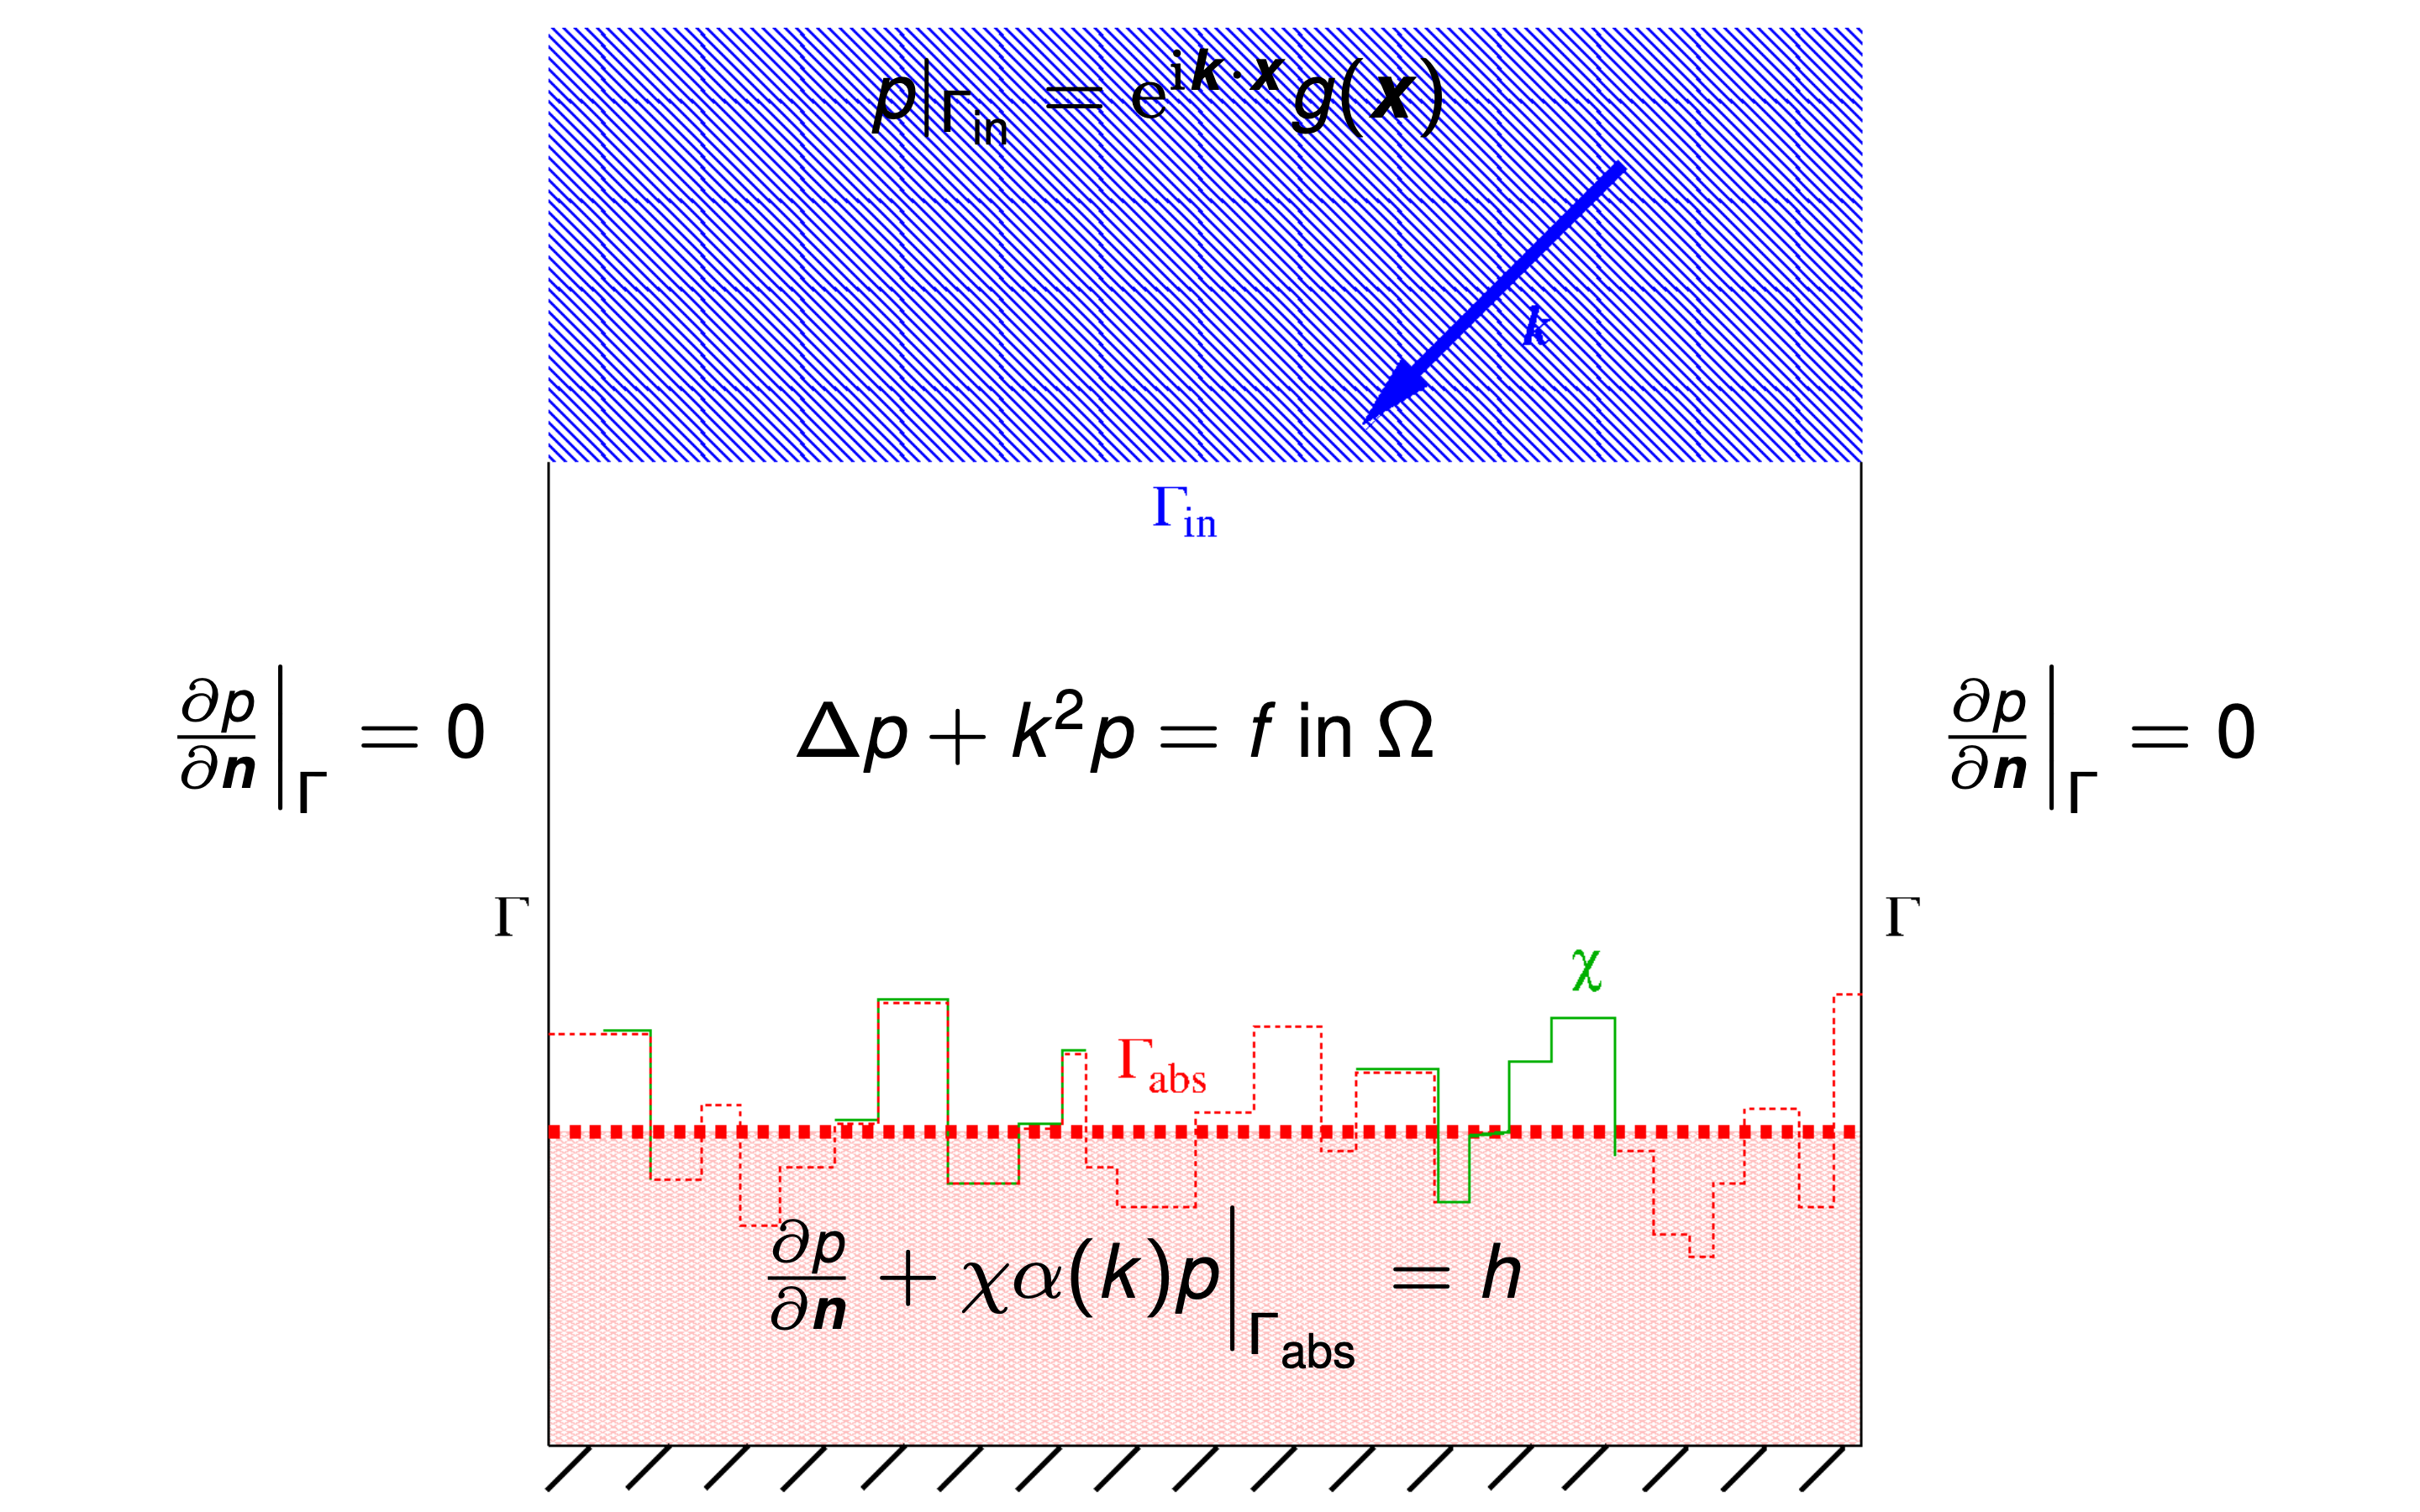
\includegraphics[width=0.55\linewidth]{Beamer/numerique/probleme.png}
            \caption{Équations dans le domaine}
            \label{fig:enter-label}
        \end{figure}
\end{frame}

\begin{frame}{Présentation du problème}
    Ceci nous amène au système suivant:
    \begin{equation}
        \tag{P_\chi}
        \begin{cases}
        \Delta p + k^2 p = 0 \text{ dans } \Omega \\
        p = g_{in} \text{ sur } \Gamma_{in} \\
        \displaystyle \frac{\partial p}{\partial n} = 0 \text{ sur } \Gamma \\[5pt]
        \displaystyle \frac{\partial p}{\partial n} + \alpha \chi p = 0 \text{ sur } \Gamma_{abs}
        \end{cases} 
    \end{equation}
    Variables :
    \begin{itemize}
        \item $\alpha$ est le coefficient d'absorption du lineur, il dépend du matériau;
        \item $\chi : \Gamma_{abs} \to \{0,1\}$ est la fonction caractéristique du lineur;
        \item $k$ est le nombre d'ondes.
    \end{itemize}
\end{frame}

\begin{frame}{Présentation du problème}
    • Nous avons une quantité fixée du matériaux atténuant le niveau sonore. Cette quantité est $\displaystyle \int_{\Gamma_{abs}}\chi dS = \beta$. \\ \\
    • Nous voulons diminuer le niveau sonore dans notre domaine, c'est-à-dire, diminuer l'énergie. L'expression de l'énergie $J$ est donnée par:
    $$J(\chi) := \int_\Omega |p_\chi|^2dx$$
    où $p_\chi$ est la solution du système de Helmhholtz dans le réacteur ëen fonction de la répartition de liner $\chi$.
\end{frame}

\begin{frame}{Calcul de l'énergie}
    \small
    • Approximation de l'aire expliquée dans \cite{4}:
    $$\displaystyle \int_a^b \int_c^d f(x,y)dy dx = [f(a,c) + f(a, d) + f(b, c) + f(b, d)]\frac{(b-a)(d-c)}{4} + E(f)$$ avec $E(f)$ l'erreur qui dépend des conditions sur $f$.\\ \\
    • L'algorithme utilisé :
    \begin{itemize}
        \item  \vskip -0.2cm Prendre un point du maillage qui possède un voisin à droite et en bas;
        \item Regarder si le carré formé par le point initial, son voisin en bas, son voisin à droite et son voisin en bas à droite est dans l'intérieur du domaine;
        \item Si c'est le cas, calculer la moyenne de la valeur absolue au carré des points du carré;
        \item Multiplier cette moyenne par l'aire du carré, cela nous donne une approximation de l'énergie dans le carré;
        \item Faire ceci pour tous les points qui ont un voisin à droite et en bas.
    \end{itemize}
\end{frame}

\begin{frame}{Algorithme du gradient}
    • But : minimiser une fonction réelle différentiable dans un espace euclidien.\\ \\
    La fonction à minimiser est $ \chi \mapsto J(\chi)$. $J$ est bien différentiable au sens de Fréchet avec $J'(\chi) : L^{\infty}(\Gamma_{abs}) \to L^1(\Gamma_{abs})$ telle que:
    $$J(\chi + \chi_0) = J(\chi) + \langle J'(\chi), \chi_0 \rangle + o(\chi_0)\,, \lim_{||\chi_0||_{\infty} \to 0} \displaystyle \frac{|o(\chi_0)|}{||\chi_0||_{\infty}} = 0.$$
    Avec $\textcolor{blue}{J'(\chi) = - \text{Re}(\alpha p_\chi q_\chi)}$ où $q_\chi$ est la solution du système adjoint de $(P_\chi)$:
    \begin{equation}
        \tag{P'_\chi}
        \begin{cases}
        \Delta q + k^2 q = -2\bar{p_\chi} \text{ dans } \Omega \\
        q = 0 \text{ sur } \Gamma_{in} \\
        \displaystyle \frac{\partial q}{\partial n} = 0 \text{ sur } \Gamma \\[5pt]
        \displaystyle \frac{\partial q}{\partial n} + \alpha \chi q = 0 \text{ sur } \Gamma_{abs}
        \end{cases}
    \end{equation}
\end{frame}

\begin{frame}{Algorithme du gradient}
    L'algorithme du gradient nous amène à considérer :
$$ \chi^{(k+1)} = \mathcal{P}_{\ell_k}\big[\chi^{(k)} - \mu_k J'(\chi^{(k)})\big]$$
où $\mathcal{P}_{\ell_k}$ est un projecteur et $\mu_k > 0$ est le taux d'apprentissage.\\ \\
Si à l'itération $k+1$ nous n'arrivons pas à diminuer l'énergie par rapport à l'itération $k$, nous divisions par $2$ le taux d'apprentissage $\mu_k$ et nous recalculons $\chi^{(k+1)}$. Cependant si l'énergie est bel et bien diminuée, alors on ajoute $\epsilon_3$ à $\mu_k$, avec $\epsilon_3$ un réel suffisamment petit.
\end{frame}

\begin{frame}{Algorithme du gradient}
    Le schéma est bien convergent vers un minimum car à chaque étape l'énergie décroît théoriquement, $\forall k > 0$:
    \small
    \begin{align*}
        J(\chi^{(k+1)}) - J(\chi^{(k)}) &= J(\chi^{(k)}) + \langle J'(\chi^{(k)}), -\mu_k J'(\chi^{(k)}) \rangle - J(\chi^{(k)}) + o(\mu_k J'(\chi^{(k)}))\\ 
        &= -\mu_k ||J'(\chi^{(k)})||^2 + o(\mu_k J'(\chi^{(k)})).
    \end{align*}
    \normalsize et,
    \begin{align*}
        \lim_{||\mu_k J'(\chi^{(k)})||_{\infty} \to 0} \displaystyle \frac{|o(\mu_k J'(\chi^{(k)}))|}{||\mu_k J'(\chi^{(k)})||_{\infty}} &= \lim_{\mu_k \to 0} \displaystyle \frac{|o(\mu_k J'(\chi^{(k)}))|}{||\mu_k J'(\chi^{(k)})||_{\infty}} \\
        &= \lim_{\mu_k \to 0} \displaystyle \frac{|o(\mu_k J'(\chi^{(k)}))|}{|\mu_k||| J'(\chi^{(k)})||^2_{\infty}} \\
        &= 0.
    \end{align*}
\end{frame}

\begin{frame}{Projecteur}
    Objectif : garantir $\chi^{(k+1)}$ dans $[0, 1]$ et $\beta = \displaystyle \int_{\Gamma_{abs}}\chi^{(k+1)}  dS$. \\ \\
    • Le projecteur choisi est $\mathcal{P}_{\ell}(\chi) = \max(0, \min(\chi + \ell, 1))$.\\ \\
    • Comme $\ell \mapsto \displaystyle \int_{\Gamma_{abs}}\max(0, \min(\chi + \ell, 1))dS$ est croissante, il est possible de faire une dichotomie pour trouver $\ell$.\\ \\
    • Les bornes utilisées pour $\ell$ sont $-\max(\chi)$ et $1$ car
    $$\displaystyle \int_{\Gamma_{abs}}\max(0, \min(\chi - \max(\chi), 1))dS = 0$$ et, $$\displaystyle \int_{\Gamma_{abs}}\max(0, \min(\chi + 1, 1))dS = 1.$$
\end{frame}

\begin{frame}{Problèmes rencontrés}
    \begin{itemize}
        \item Finesse du maillage;
        \item Sortie trop précipitée de la grande boucle;
        \item Non convergence vers un minimum.
    \end{itemize}
    \begin{figure}
        \centering
        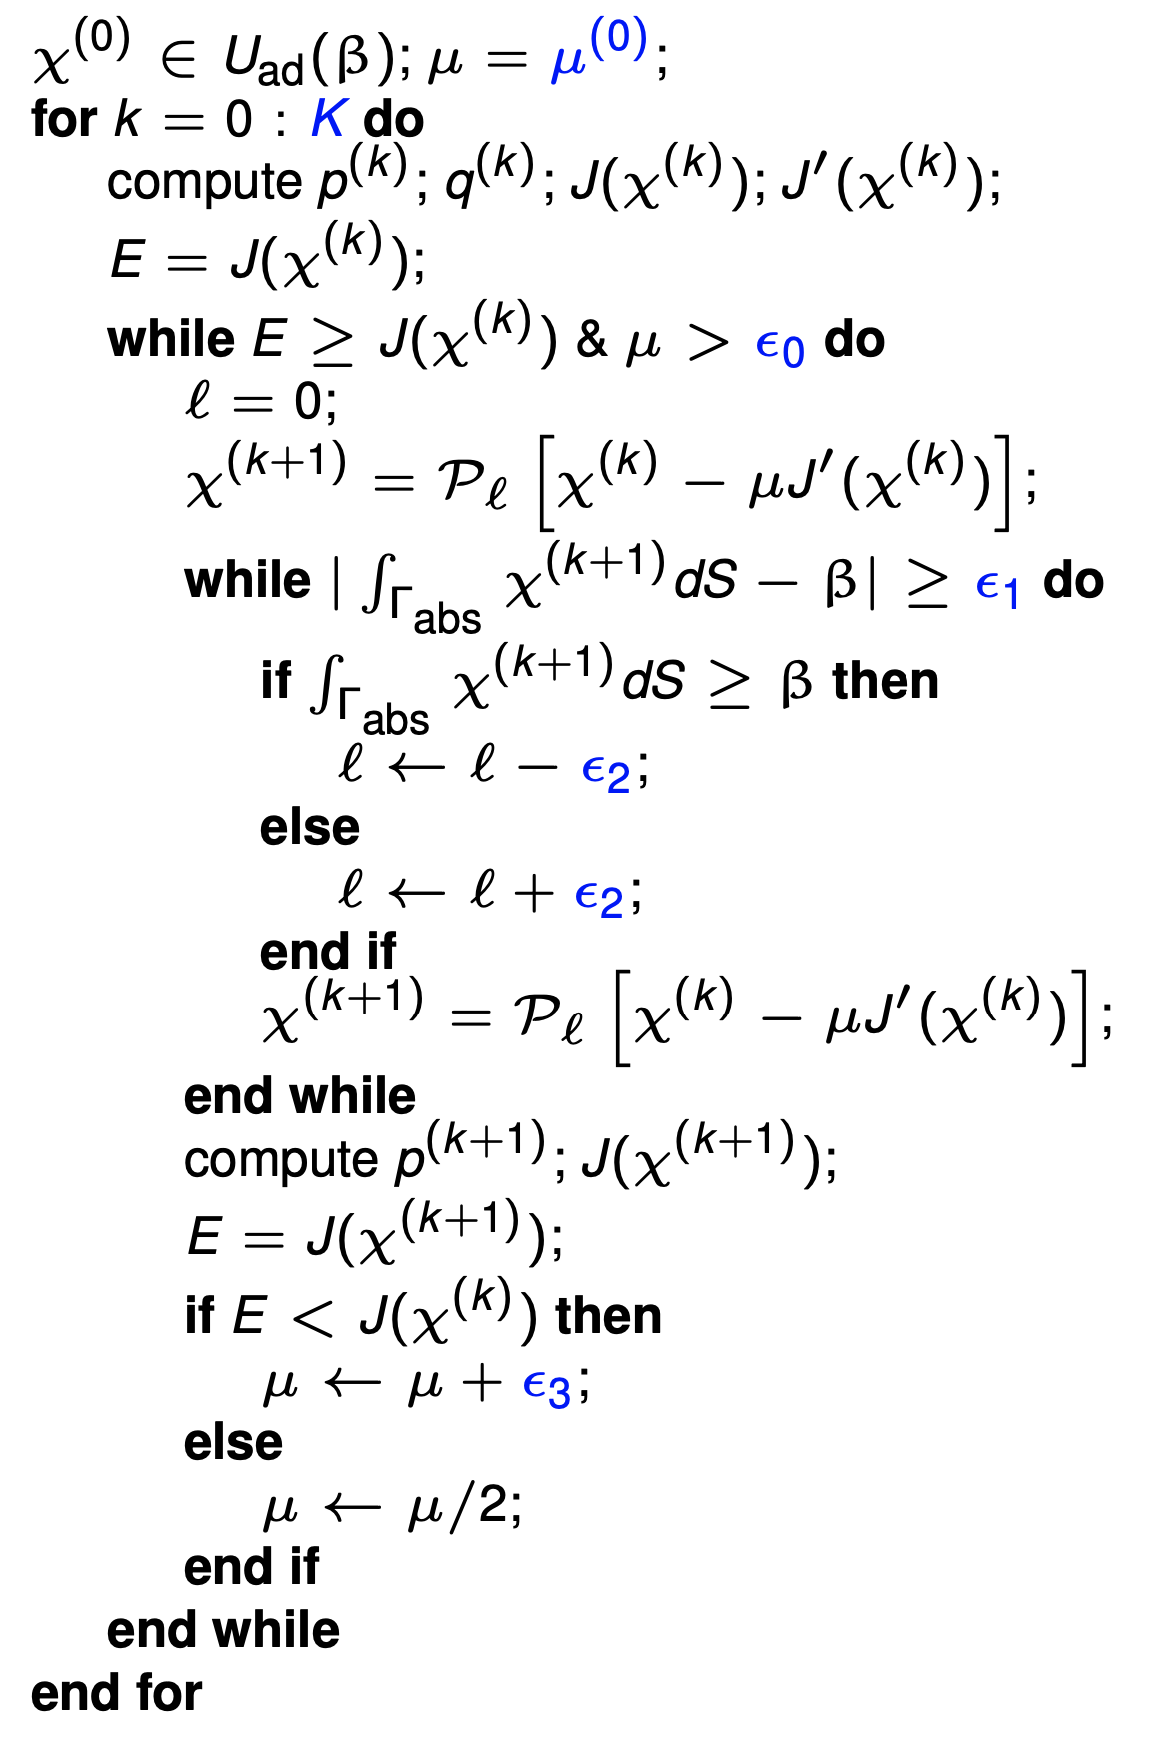
\includegraphics[width = 0.3\linewidth]{Beamer/pseudo_code.png}
        \caption{Pseudo code de l'algorithme de gradient}
        \label{fig:enter-label}
    \end{figure}
\end{frame}

\begin{frame}{Solutions proposées}
    \begin{itemize}
        \item Enlever la condition sur $\mu_k$ pour sortir des boucles;
        \item Rajouter $10^{-3}$ à $\mu_k$ à chaque passage dans la grande boucle;
        \item Rajouter un nombre max d'itérations dans la petite boucle.
    \end{itemize}
    \begin{figure}
        \centering
        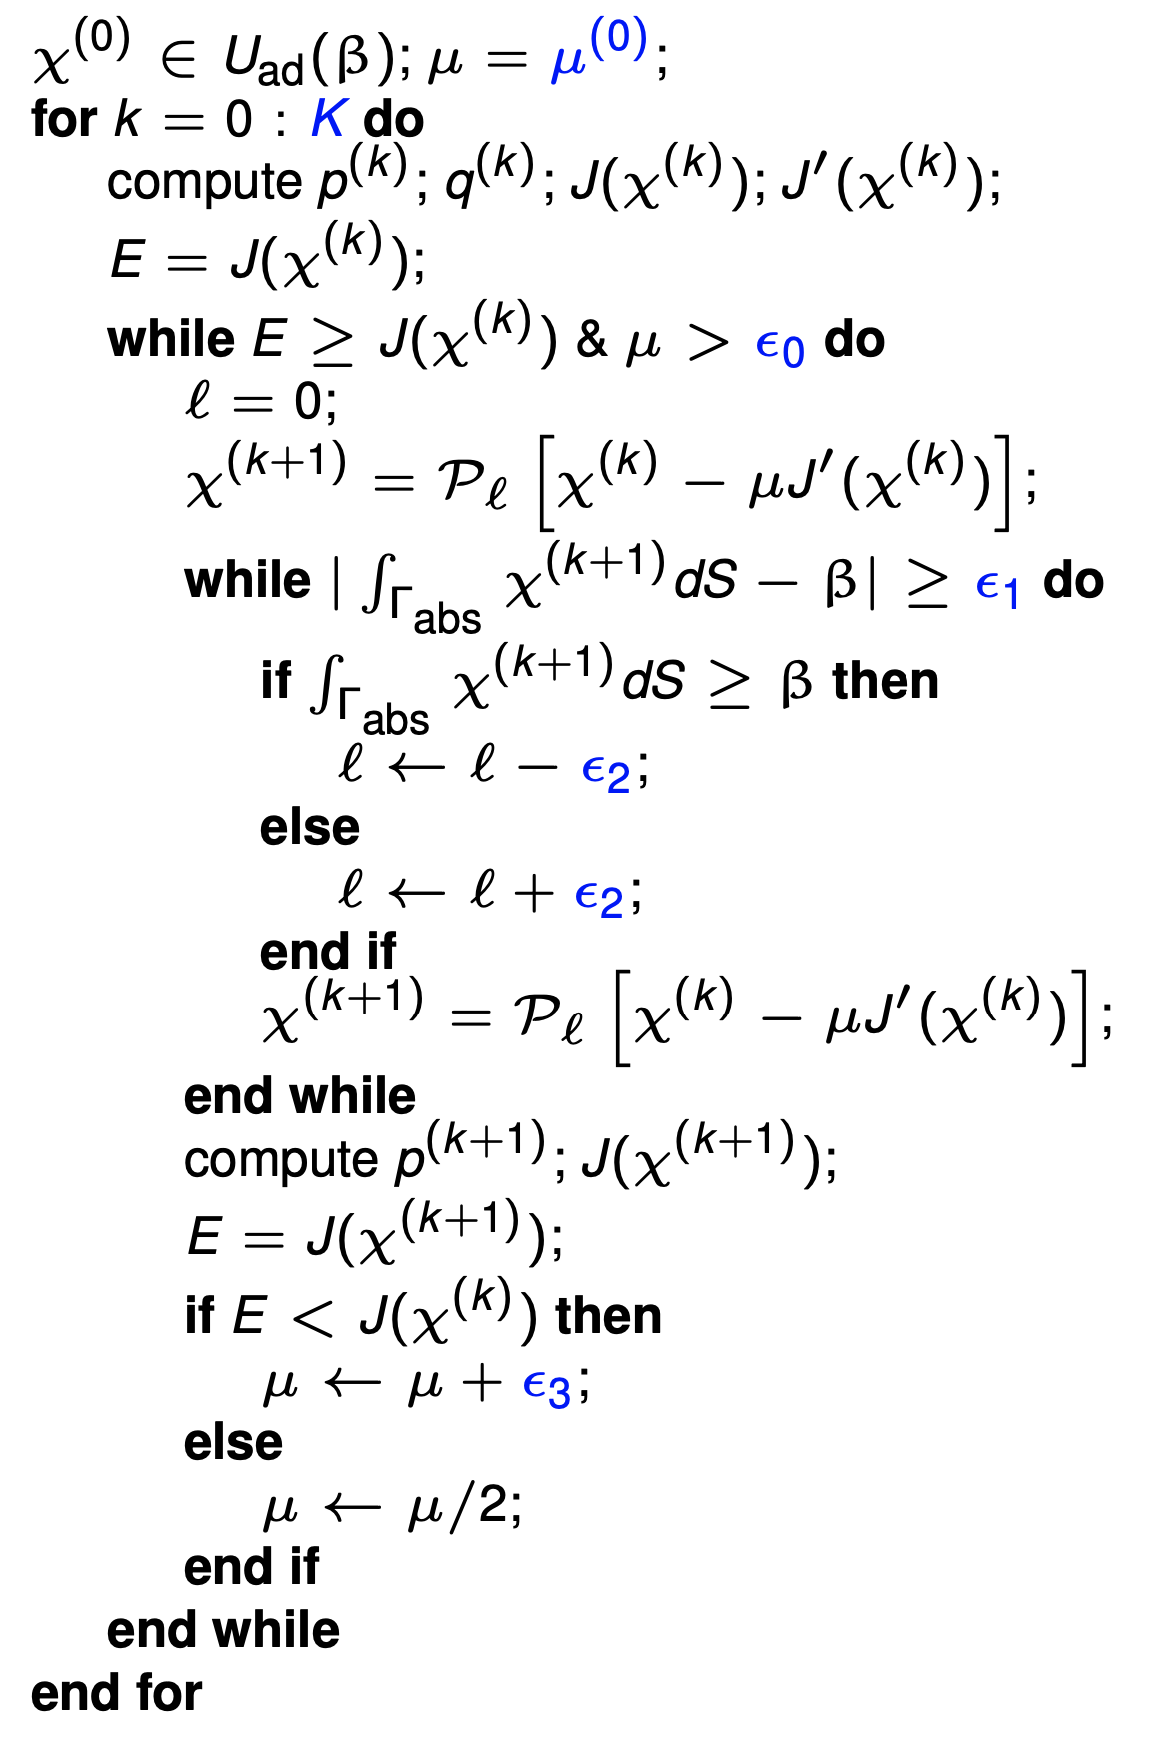
\includegraphics[width = 0.3\linewidth]{Beamer/pseudo_code.png}
        \caption{Pseudo code de l'algorithme de gradient}
        \label{fig:enter-label}
    \end{figure}
\end{frame}

\begin{frame}{Analyse des résultats}
    Afin de développer la meilleure solution pour la réduction de l'intensité sonore, nous avons fait plusieurs études numériques :
    \begin{itemize}
        \item Étude de la géométrie;
        \item Étude des matériaux,
        \item Étude de la quantité de liners
        \item Étude de la fréquences des ondes à atténuer.
    \end{itemize}
\end{frame}
\begin{frame}{Intervalle de fréquence considéré}
    Les bruits créés par les moteurs d’avion proviennent de trois sources principalement : 
    \begin{itemize}
        \item le ventilateur;
        \item la turbine;
        \item la combustion.
    \end{itemize}
    La combinaison de ces bruits se situe entre 100 Hz et 6 000 Hz. Étant donné que $ k = \omega/c = 2\pi f/c$, nous allons donc étudier le problème pour $k \in [1.85\,m^{-1}, 112\,m^{-1}].$ 
\end{frame}

\begin{frame}{Étude de la géométrie}
    • On étudie l'efficacité de l'atténuation d'une frontière plane et d'une frontière comportant une fractale de niveau 1, puis 2, puis 3, totalement absorbant ($\beta=1$). \\
    
    \begin{table}
        \centering
        \begin{tabular}{cccc}
            Fractale & Énergie Max  & Énergie Moyenne\\
             Niveau 0& 16,7 & 1,2 & \\
             Niveau 1 & 5,0 & 0,94 & \\
             Niveau 2 & 3,37 & 0,75 & \\
             Niveau 3 & 3,35 & 0,6 & \\
        \end{tabular}
        \label{tab:my_label}
    \end{table}

\vskip 1cm
$\to$ Les fractales de niveau 2 et 3 sont donc les plus efficaces.
\end{frame}

\begin{frame}{Étude des matériaux}
\begin{figure}[H]
    \centering
    \subfloat{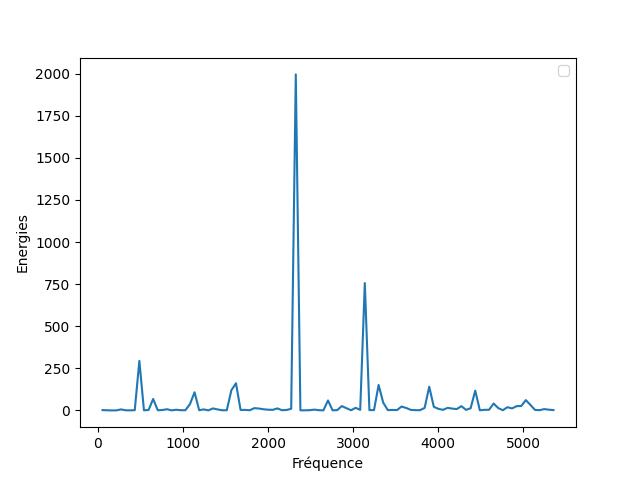
\includegraphics[width = 1.5in]{Beamer/numerique/Level_2_Alpha_refle.png}}
    \subfloat{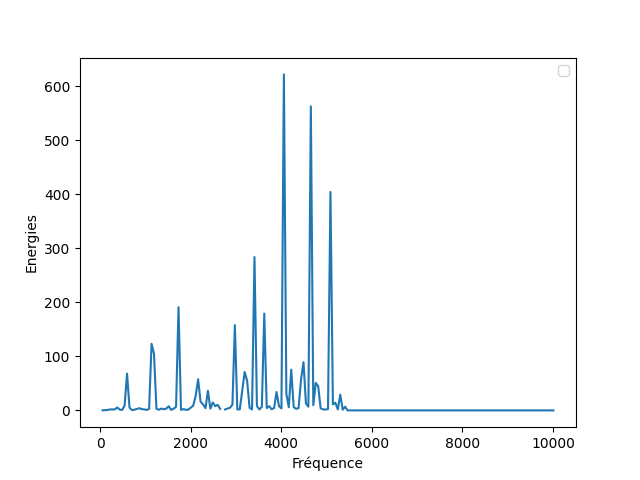
\includegraphics[width = 1.5in]{Beamer/numerique/Level_3_Alpha_refle.png}}\\
    \caption{\tiny Énergie en fonction de la fréquence avec un matériau réfléchissant ($\alpha = 10 - 0.10j$)}
    \label{freq}
\end{figure}
\begin{figure}[H]
    \centering
    \subfloat{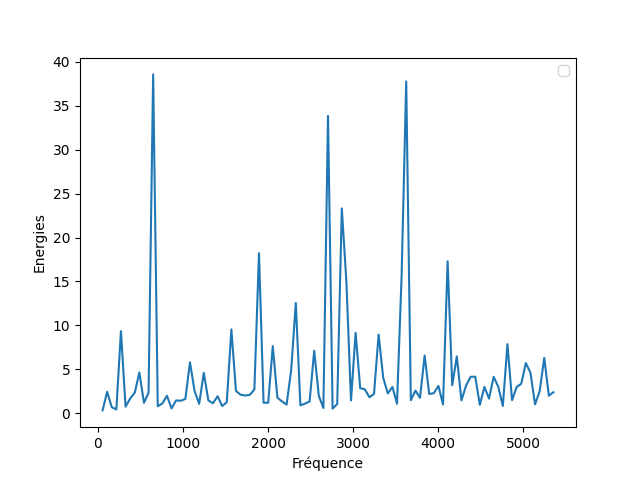
\includegraphics[width = 1.5in]{Beamer/numerique/Level_2_Alpha_absorp.png}}
    \subfloat{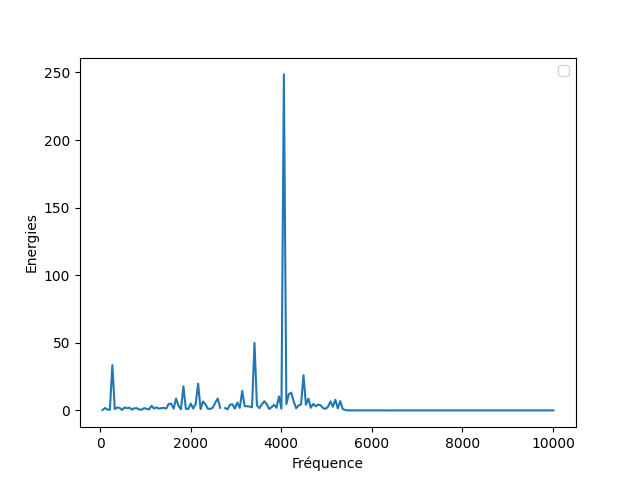
\includegraphics[width = 1.5in]{Beamer/numerique/Level_3_Alpha_Absorp.png}}\\
    \caption{\tiny Énergie en fonction de la fréquence avec un matériau absorbant ($\alpha = 10 - 10j$)}
    \label{freq}
\end{figure}
\end{frame}

\begin{frame}{Étude de la quantité de matériaux}
    • On étudie l'efficacité de l'atténuation en fonction de la quantité de matériaux utilisé par le liner afin de trouver le meilleur compromis entre atténuation et coût.
    \begin{figure}[H]
    \centering
    \subfloat{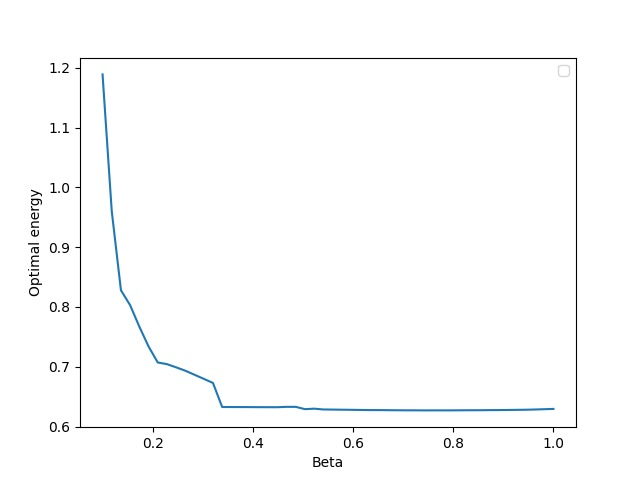
\includegraphics[width = 1.8in]{Beamer/numerique/qt1.jpeg}}
    \subfloat{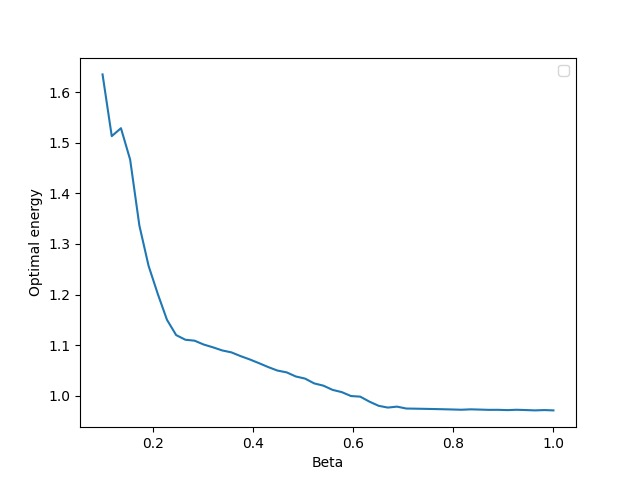
\includegraphics[width = 1.8in]{Beamer/numerique/qt2.jpeg}}\\
    \caption{\tiny Énergie après optimisation en fonction de $\beta$ pour la fractale de niveau 2 et 3}
    \label{freq}
\end{figure}
    Par exemple pour une paroi en fractale de niveau 2, on choisit $\beta = 0.4$.
\end{frame}
\begin{frame}{Étude de la fréquence des ondes à atténuer}
    • Optimisation des 20 énergies les plus grandes. On obtient les résultats suivants:
        \begin{figure}[H]
        \centering
        \subfloat{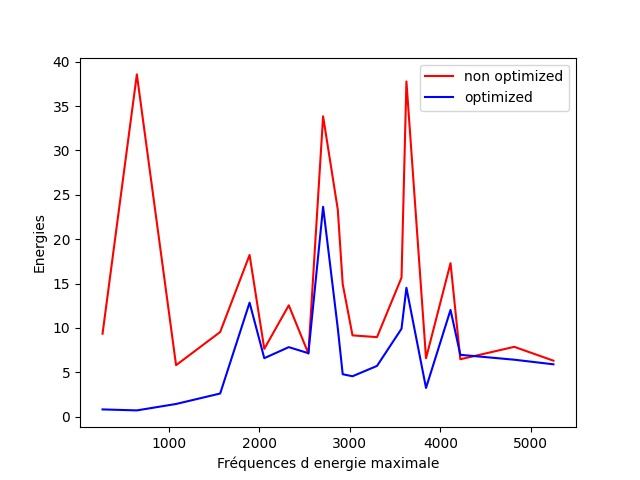
\includegraphics[width = 1.8in]{Beamer/numerique/WhatsApp Image 2023-11-16 at 21.11.41.jpeg}}
        \subfloat{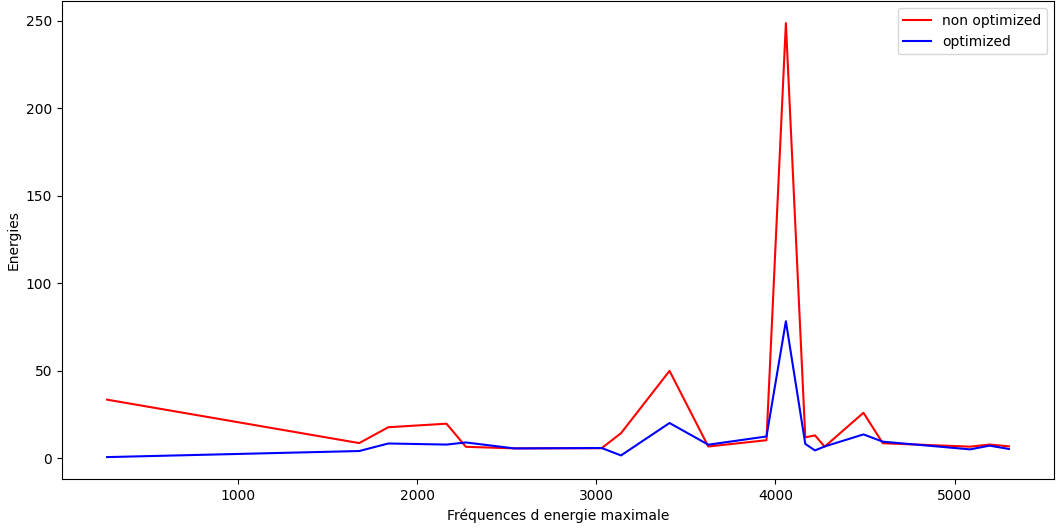
\includegraphics[width = 2.4in]{Beamer/numerique/LEVEL3.png}}\\
        \caption{Énergie après optimisation en fonction de f pour la fractale de niveau 2 et 3}
        \label{freq}
    \end{figure}

\end{frame}
\begin{frame}{Optimisation multi-fréquentielle}
    On cherche maintenant à optimiser pour l'ensemble des fréquences problématiques simultanément. Les modifications dans l'algorithme sont : 
    \begin{itemize}
        \item Une nouvelle fonction de coût $J$;
        \item Un nouveau gradient.
    \end{itemize}
\end{frame}


\begin{frame}{Optimisation multi-fréquentielle}
    La nouvelle fonction de coût ne sera plus l'énergie
        $$J(\chi) := \int_\Omega |p_\chi|^2$$
    car $p_\chi$ est la solution de l'équation de Helmholtz pour une fréquence $f$ bien déterminée. On utilisera plutôt une somme pondérée par la famille $(\lambda_k)$ des énergies relatives à chaque fréquence considérée:
    \textcolor{blue}{$$J(\chi) := \sum_{k} \lambda_{k} \int_\Omega |p_{k_{\chi}}|^2$$}
    où $k$ parcourt les fréquences problématiques et $p_{k_{\chi}}$ est la solution de l'équation de Helmholtz pour le nombre d'onde $k$.
    Le nouveau gradient devient:
    \textcolor{blue}{$$J'(\chi) := - \sum_{k} \lambda_{k} \text{Re}(\alpha p_{k} q_{k}).$$}
\end{frame}
\begin{frame}{Optimisation multi-fréquentielle} 
    Comparaison entre les différentes énergies non optimisées et optimisées avec les différentes méthodes:
    \vskip -0.1cm
    \begin{figure}
        \centering
        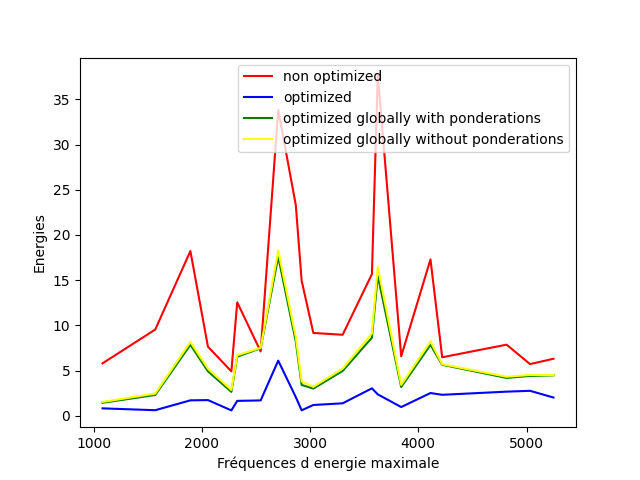
\includegraphics[width=0.65\linewidth]{Beamer/comparaisons.png}
        \vskip -0.2cm
        \caption{\tiny Comparaison entre l'optimisation mono et multi-fréquentielle.}
        \label{fig:enter-label}
    \end{figure}
\end{frame}
\begin{frame}{Autre méthode d'optimisation : approche stochastique}
• Méthode hill-climbing : partir d'un $\chi$ aléatoire puis explorer itérativement son voisinage pour essayer de trouver une meilleure solution.\\


• Expérimentalement : peu importe le nombre d'itération, on trouve toujours une solution d'efficacité semblable.

\end{frame}


\begin{frame}{Autre méthode d'optimisation : approche stochastique}
\begin{figure}[H]
    \centering
    \subfloat{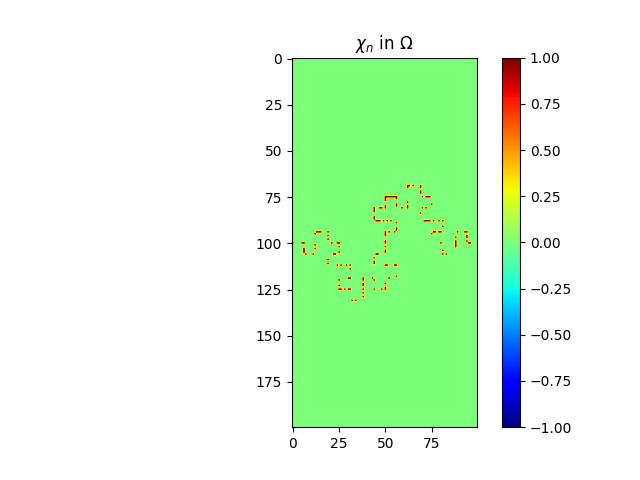
\includegraphics[width = 1.5in]{Beamer/assets/rand/chi_rand_2.jpg}}
    \subfloat{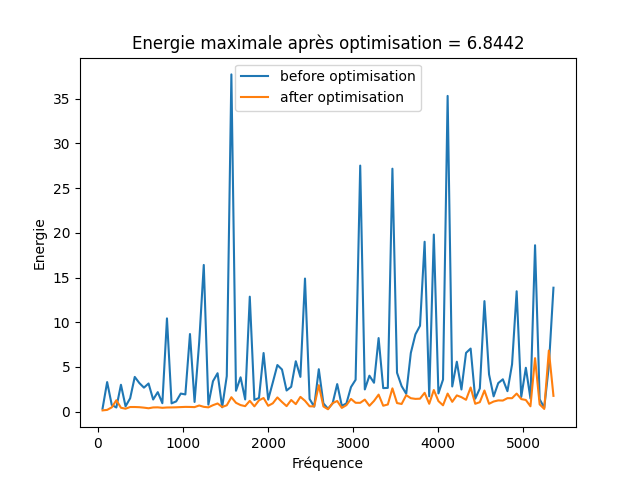
\includegraphics[width = 1.5in]{Beamer/assets/rand/level2_rand.png}}\\
    \caption{\tiny Optimisation stochastique avec fractale de niveau 2}
    \label{freq}
\end{figure}
\begin{figure}[H]
    \centering
    \subfloat{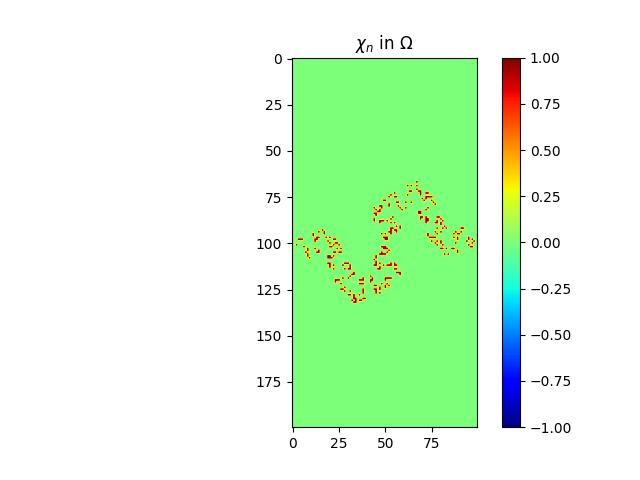
\includegraphics[width = 1.5in]{Beamer/assets/rand/chi_rand_3.jpg}}
    \subfloat{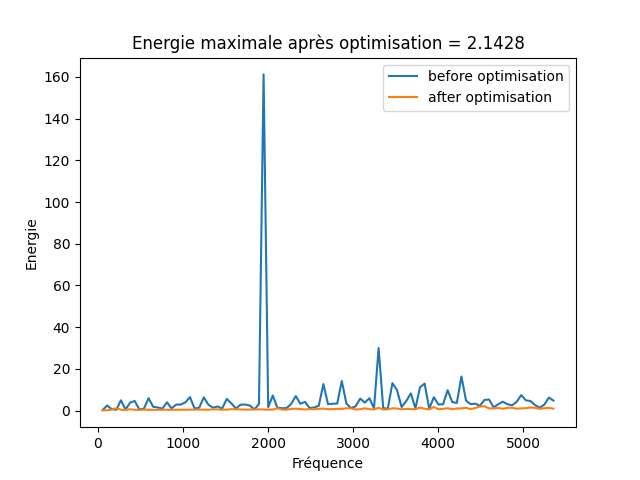
\includegraphics[width = 1.5in]{Beamer/assets/rand/rand_level3.png}}\\
    \caption{\tiny Optimisation stochastique avec fractale de niveau 3}
    \label{freq}
\end{figure}
\end{frame}

\begin{frame}{Solution retenue}
    \begin{figure}[H]
    \centering
    \subfloat{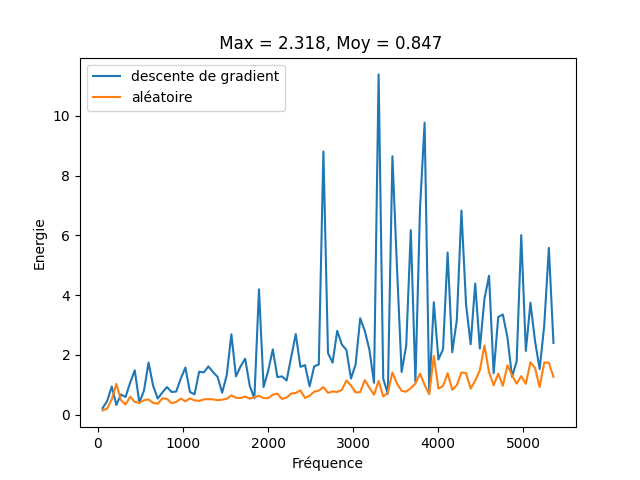
\includegraphics[width = 2.2in]{Beamer/numerique/chifinal.png}}
    \subfloat{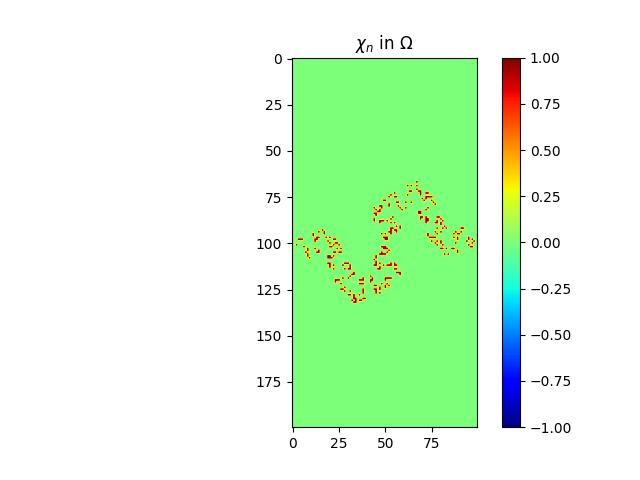
\includegraphics[width = 2.2in]{Beamer/assets/rand/chi_rand_3.jpg}}\\
    \caption{\tiny Comparaison avec l'algorithme de descente de gradient}
    \label{freq}
\end{figure}
Solution retenue : Fractale de niveau 3, $\beta = 0,4$, $\chi$ aléatoire.
\end{frame}

\begin{frame}{Conclusion numérique}
    Résumé de notre démarche:
    \begin{itemize}
        \item Implémentation d'un algorithme de descente de gradient;
        \item Plusieurs études pour choisir des paramètres adaptés;
        \item Comparaison de l'efficacité avec un algorithme stochastique;
    \end{itemize}
    \vskip 0.9 cm
    Améliorations possibles : 
    \begin{itemize}
        \item Meilleur ajustement des hyperparamètres (learning rate);
        \item Explorer d'autres algorithmes d'optimisation (algorithme génétique...).
    \end{itemize}
\end{frame}

\begin{frame}
    \begin{center}
    \Huge \textcolor{faeng_blue}{Merci !} 
    \end{center}
\end{frame}

\begin{frame}{Bibliographie}
    \nocite{*}
    \printbibliography[]
\end{frame}
\end{document}
